\section{Project Design}\label{sec:4}

This chapter presents the design of TraceAdvisor and the reasoning behind it. Section~\ref{sec:2} introduced the subsystems and how they connect; here each design decision is stated together with the problem it addresses, the alternatives considered and the reasons for the choice. Implementation details and measured outputs follow in Section~\ref{sec:5}.

Three requirements shape the design. The first is pre-execution validity: a recommendation may use only information available before the run it sizes, because any path by which future information reaches a recommendation, directly or through the evaluation procedure, produces results that cannot be achieved in practice. The second is asymmetric risk: a job whose memory is exceeded can be killed and rerun, whereas an over-provisioned job only wastes capacity, so under- and over-provisioning must be treated separately rather than averaged. The third is dataset heterogeneity: production traces differ in what they record, at what level and in which units \cite{ref7,ref19}, and policies must be compared fairly within each dataset without assuming that the datasets measure the same thing.

These requirements also position TraceAdvisor relative to existing approaches, which are reviewed in Section~\ref{sec:1}. Runtime resource managers reclaim slack after jobs have been admitted, inside provider-controlled infrastructure, and leave the submission-time request unchanged; configuration optimizers search for good configurations through repeated online experimentation. TraceAdvisor instead acts at submission and learns only from historical traces, so it needs neither scheduler modification nor online profiling. Because no recommendation can be tested live, the credibility of the system rests on an offline evaluation that faithfully reproduces the information available at submission time, and much of the design serves that purpose.

\subsection{Data Pipeline Design}\label{sec:4.1}

The data pipeline turns two structurally different traces into evaluation rows that later stages can treat identically. Its central decision is to confine dataset-specific logic to the start of the pipeline and to make the meaning of every value explicit where the datasets meet. Fig.~\ref{fig:4.1} shows the two ingestion paths.

\begin{figure*}[!t]
\centering
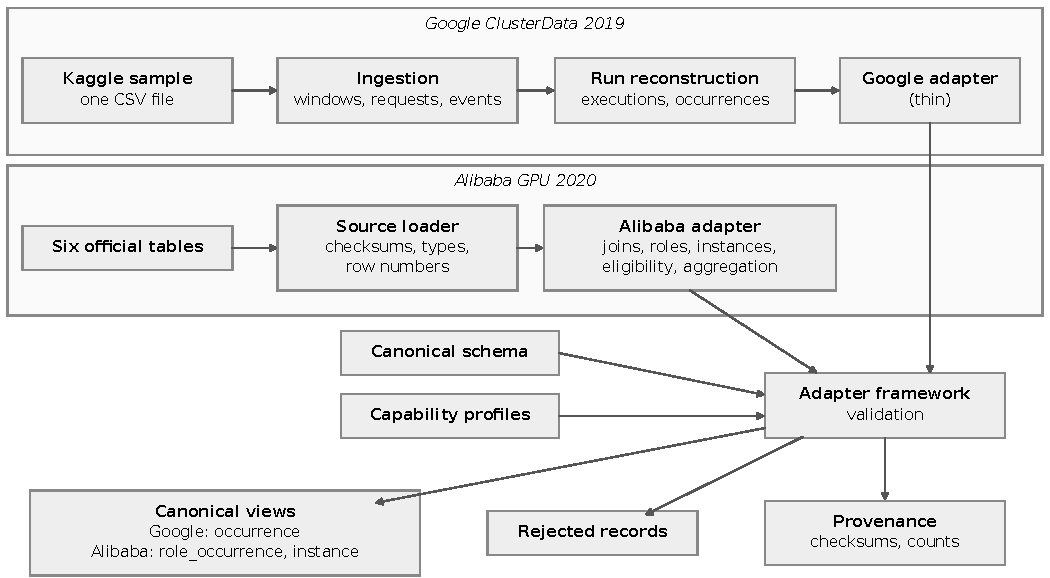
\includegraphics[width=0.92\linewidth]{figures/fig_4_1.pdf}
\caption{Data ingestion and canonicalization}\label{fig:4.1}
\end{figure*}

\subsubsection{Canonical Data Model}\label{sec:4.1.1}

Google ClusterData 2019 records task usage in short time windows with normalized resource values \cite{ref7}, whereas the Alibaba GPU 2020 trace records jobs, task roles and instances with lifetime summaries in physical units \cite{ref19}. A separate pipeline per dataset would duplicate the splitting, history, recommendation and evaluation logic, and any divergence between the copies would undermine cross-dataset conclusions. Converting both datasets to common physical units is not possible, because the publisher normalizes the Google values. The adopted design therefore maps each dataset into one canonical data model that standardizes field names and record levels while keeping each dataset's units and semantics explicit.

Four rules govern the model, each preventing a specific error. Requests, observed averages, observed peaks, targets and recommendations are stored as separate fields, because an average never exceeds its peak, and evaluating against average usage where the peak determines failure would understate every violation rate. Every value carries its unit, and a request must share a unit with the corresponding usage, so that ratios and differences are well defined; values keep their source scale, which preserves traceability. Missing values are never replaced with zero: a missing actual value set to zero could never be violated, and a missing history set to zero would tell a model that a workload used no resources. Finally, data quality is recorded per resource, eligibility as an exclusion reason and dataset capability in a profile, because a single validity flag would, for example, discard a valid memory measurement whenever the CPU value is missing.

\subsubsection{Dataset Capability Profiles}\label{sec:4.1.2}

Each dataset declares a capability profile that states its supported resources, whether CPU is recorded as a peak or an average, the unit of each resource, the evaluated record level, whether a combined CPU-or-memory metric is meaningful, and whether targets must stay within one split. The profile is consulted when adapter output is validated, when targets are built and when results are reported. The alternative, dataset-specific conditions scattered through shared code, would allow a new dataset to be evaluated under assumptions that hold only for another; the profile declares a dataset's properties once and enforces them throughout.

\subsubsection{Dataset Preparation and the Adapter Framework}\label{sec:4.1.3}

All processing that depends on the source format, namely parsing, joins, timestamp conversion, unit tagging, recurrence and occurrence construction, eligibility, aggregation and traceability, belongs to the dataset-preparation layer. On Google, runs are reconstructed before the adapter; on Alibaba, roles and instances are built within it. Neither preparation code nor adapters may compute splits, history, targets, recommendations or metrics, and the framework rejects any adapter output that contains split labels or targets. This boundary guards against leakage, the use of information unavailable at prediction time, which is a common cause of overly optimistic results, and it ensures that all time-dependent logic is implemented and tested once, in shared code.

The framework offers a single-table path for sources delivered as one table and a multi-table path that joins several tables and produces several validated views and a rejected output. Every source row must appear in a view or in the rejected output, and counts are reconciled before publication, so any loss of data is detected. Because the Google pipeline predates the framework and its results had already been validated, its reconstruction logic was not migrated into an adapter. A thin adapter instead maps the occurrences it produces into the canonical form, and an acceptance test requires the result to equal the existing Google canonical view.

\subsubsection{Evaluation Units}\label{sec:4.1.4}

A recommendation must be produced for the unit for which a user requests resources; otherwise it answers a different question from the one the user faces. In the Google trace, the tasks of a job are submitted together as one collection and share its request \cite{ref7}, so the unit is the full workload occurrence: executions of the same workload that start together. Because these executions run in parallel, their usage is summed within each aligned time window and the maximum of this sum is the occurrence peak. The sum of individual peaks was rejected because tasks rarely peak simultaneously, so it would overstate the combined peak.

An Alibaba job comprises roles, such as workers and parameter servers, with very different resource profiles, so one recommendation for the whole job would suit none of them. Requests are specified per instance, so the unit is one role within one job, with values per instance. The role's memory peak is the maximum over its instances, which represents what each instance of the role requires; a sum of instance peaks was rejected because, without time-aligned usage, it is only an upper bound on the combined peak. The number of instances is treated as given and is not predicted.

\subsubsection{Workload Identity and Recurrence}\label{sec:4.1.5}

History-based recommendation depends on correctly identifying repeated runs of the same workload. Google provides no recurrence tag, so recurrence is constructed from the user and the job's logical name, which the trace provides to group executions of the same program. Alibaba provides an official \texttt{group} tag, which is combined with the task role so that the histories of different roles are kept apart. No recurrence is inferred where a dataset does not record one, because an incorrect key would merge unrelated workloads into one history; Alibaba jobs without a \texttt{group} tag keep a fallback identity for auditing but are not evaluated.

\subsubsection{Eligibility Criteria}\label{sec:4.1.6}

An Alibaba role is evaluated only when its measurements fully describe a completed run: it has a recurrence key, its job and task completed, its request is valid, every instance ran once and completed with sensor data, and its resource values are valid. Fourteen rules check these conditions in a fixed order, from job-level to task, instance, attempt, sensor and memory checks, and each ineligible role records the first rule it fails, which makes every recorded reason informative and every count deterministic. A worker that ran more than once is excluded because the sensor table holds one row per worker, which cannot be attributed to a particular attempt. A role lacking sensor data for some instances is excluded because a maximum over only some instances would be an unlabelled lower bound on its peak. Restricting evaluation to completed, fully observed runs biases the sample towards well-behaved workloads; this is accepted because evaluating against incomplete measurements would be less reliable, and it is discussed as a limitation in Section~\ref{sec:9}.

\subsubsection{Temporal Data Design}\label{sec:4.1.7}

Cluster workloads are non-stationary, and random cross-validation on time-ordered data lets a model learn from runs that occur after those it is evaluated on, which overstates accuracy. Three rules enforce temporal validity. Rows are ordered by start time and split 70/15/15 into training, validation and test sets, with boundaries only between groups of equal start time, so that runs starting together, such as the roles of one Alibaba job, are never divided. The history of a row contains only earlier eligible occurrences of the same workload that had completed at or before its start, because a run still in progress has not yet revealed its peak. The target is the usage of the next eligible occurrence, and when it is unavailable a status records why (no next occurrence, an unusable value, a next occurrence in another split or an unsupported resource), so missing targets are explained rather than silently dropped.

On Alibaba, a target must lie in the same split as its row, so validation never uses an outcome from the test period. The Google pipeline does not enforce this rule, and some Google validation targets fall in the test period. No future information enters a Google recommendation, because history and features use only earlier data, but Google validation results are somewhat optimistic; the capability profile records this limitation, and its effect is measured by a sensitivity analysis (Section~\ref{sec:4.3}).

\subsection{Recommendation Model Design}\label{sec:4.2}

Seven policies are compared. They span the status quo, simple rules used in production systems and learned models, so that any benefit of learning is measured against strong simple alternatives rather than against the user's request alone. Every choice among them is made on the training and validation sets only, and every policy is scored by the same evaluator.

\subsubsection{Historical Percentile Baselines}\label{sec:4.2.1}

For a recurring workload, its own earlier runs are the most direct evidence of what the next run will need, and production resource managers commonly size workloads from statistics of past usage, as reviewed in Section~\ref{sec:1}. History-based rules are transparent, need no training and perform well on stable workloads, so they represent what a practitioner could deploy today. The Request policy, the user's current request, is the status quo against which every other policy is measured and the fallback when no history exists. The Mean policy represents sizing for typical usage, since the mean minimizes squared error for a stable workload, and it quantifies the cost of ignoring variability: it is exceeded whenever a run is above average.

The 90th, 95th and 99th percentiles of past usage size for the tail of a workload's own distribution. If a workload's runs are assumed exchangeable, so that their order carries no information, order statistics give a direct interpretation: the probability that the next run exceeds the k-th smallest of n past values is (n + 1 $-$ k)/(n + 1). A recommendation at the q-th percentile of a long history is therefore exceeded with probability close to 1 $-$ q, so the percentile expresses the accepted risk directly. Percentiles are computed by linear interpolation between ordered values.

The same result shows the limitation of short histories. With n past runs, even the largest past value is exceeded with probability 1/(n + 1), one half after one run and one eleventh after ten, so with few runs the 99th percentile cannot deliver its nominal coverage. Each baseline therefore uses history only when a workload has at least \texttt{min\_runs} earlier runs and otherwise falls back to the request. The best threshold depends on the quality of the fallback: where requests are generous, waiting for longer history costs little, and where they are often exceeded, even a short history is better. The threshold is therefore selected on validation from 1, 3, 5 and 10. CPU and memory are handled independently, so a missing CPU history never affects a memory recommendation.

Candidates are ranked on validation by a fixed sequence of criteria rather than a weighted score, because a weighted score would require a price ratio between a violation and a unit of waste that is not known for these traces. The lexicographic ranking encodes the agreed priority, avoiding under-provisioning first and reducing waste second. On Google, where CPU and memory are both peaks, the order is the combined CPU-or-memory violation rate, the worst single-resource violation rate, the sum of both violation rates, CPU waste, memory waste and the lower \texttt{min\_runs}. On Alibaba, where memory is the primary resource, it is the memory violation rate, memory waste, CPU violation rate, CPU waste, \texttt{min\_runs} and policy name.

On Alibaba, Request is scored and reported but cannot be selected as the baseline. As the Hybrid safeguard (Section~\ref{sec:4.2.3}) it would prevent Hybrid from ever recommending below the submitted request, limiting the waste reduction Hybrid can achieve. Request also does not depend on history, so its candidates are identical across thresholds, and selecting it would fix \texttt{min\_runs} by a tie-break rather than from data.

\subsubsection{Machine Learning Forecasting}\label{sec:4.2.2}

A percentile rule uses only one workload's own history. It cannot help a workload with a short history, cannot use the request just made, and cannot learn patterns shared across workloads, such as how usage relates to request size. A regression model trained across all workloads can use this information. The task is defined as forecasting the next run's usage of each resource from information available before the current run starts, with a separate model per dataset and resource, because features, units and targets differ.

Only pre-execution information is used. On Google, the 24 features describe the occurrence's CPU and memory requests, its number of executions and the variety of their requests, the number of earlier completed occurrences, and the count, mean, standard deviation and 90th, 95th and 99th percentiles of earlier CPU peaks, memory peaks and runtimes. On Alibaba, the features are the CPU, memory and GPU requests, the number of instances, the GPU type, its specification and the workload label recorded with the job, the counts of earlier runs, and the point-in-time history statistics computed for the baselines, each with a missing-value indicator. The history statistics give the model the same information as the baselines, so it can in principle reproduce one, while the requests, counts and job descriptors add information the baselines ignore. Everything that could reveal the outcome is excluded, including targets, current-run measurements, split labels, exclusion and validity fields and identifiers, and a check rejects any feature list that contains an excluded column, so that the exclusion does not rely on convention.

The data are tabular, the features mix requests, counts, statistics and categorical job descriptors on very different scales, and the relationship between features and usage is non-linear and heavy-tailed. Tree-based models suit these conditions: they are invariant to monotone rescaling, capture non-linear effects and interactions without manual feature engineering, and work well on medium-sized tabular data. Deep sequence models were not adopted because most workloads have too few occurrences to learn per-workload sequences, and the Google training set has only a few thousand. The candidates represent distinct bias-variance trade-offs. A decision tree is the simplest non-linear model and easy to interpret, but high in variance. A random forest averages many decorrelated trees, which reduces variance and makes it robust to hyperparameter choices. Gradient-boosted trees fit trees sequentially to earlier residuals, which reduces bias; XGBoost is used on both datasets for its regularized objective, and histogram-based gradient boosting is also compared on Alibaba GPU 2020, where binning feature values makes training efficient on several hundred thousand rows. A constant predictor always predicts one value from the training data. It has no predictive skill and is the floor that a selected model must beat; without it, an accuracy figure has no reference point. On both datasets it is reported but never selected.

Next-run usage is strongly right-skewed, and with squared error on raw values the few largest workloads dominate training. On Google, models are therefore trained on log(1 + usage), which makes errors approximately relative, and predictions are transformed back with exp($\cdot$) $-$ 1. This back-transformation biases predictions low, towards the median, which the design accepts deliberately: protection against under-prediction is the task of the Hybrid safeguard, not of the accuracy-oriented model. Negative predictions are clipped to zero on both datasets.

Missing history statistics are informative, because they signal a new or rarely seen workload, and both designs preserve that information. On Google, missing values are passed to models that handle them natively. On Alibaba, a missing-value indicator is added for each history statistic before the statistic is filled with zero, so that zero usage and absent history remain distinguishable. Imputing a typical value was rejected because it would make a new workload look like an average one.

On Google, a row is used for fitting only when its target starts at or before the end of the period the model may learn from, which is the end of training during model selection and the end of validation for the final refit, so no training label comes from a period on which the model is evaluated. On Alibaba, the CPU model is trained only on rows with an available CPU target and the memory model only on rows with an available memory target, so that a missing CPU value never removes a row from memory training.

On Google, hyperparameters are chosen by grid search with time-series cross-validation on the training set. A training row near a fold boundary can have its target inside the following validation fold, so such rows are purged from the fold's training data, a technique known as purged cross-validation. A second cross-validation grouped by workload is reported as a check of generalization to unseen workloads but is not used for any decision. On Alibaba, which has far more rows, each model family is used with one fixed configuration, fitted on the training set and scored on the validation set, which preserves time order. On Google, small, explicit grids were preferred to adaptive search methods for reproducibility: every evaluated configuration is recorded.

On Google, the selected model for each resource is the candidate with the lowest validation root mean squared error on the log-transformed target, with mean absolute error on the original scale as the only tie-breaker. On Alibaba, the selected model is the candidate with the lowest validation root mean squared error, followed by mean absolute error, with violation rate and average shortfall used only to break remaining ties. Selecting by violation rate was rejected because it rewards over-prediction: a model that systematically predicts too high has few violations, and a violation-first ranking would select the constant predictor, which has no skill. Keeping an accurate model separate from the safety rule makes the source of any improvement identifiable.

Training models to predict a high quantile of next-run usage directly, by quantile regression, was considered and not adopted. A model per quantile level would multiply the number of models to tune and validate, and coverage on non-stationary data is not guaranteed without further calibration, whereas an accurate point forecast combined with an explicit historical floor gives a rule whose effect can be stated exactly (Section~\ref{sec:4.2.3}). Direct quantile modelling is discussed as future work in Section~\ref{sec:9}.

After selection, the chosen model for each resource is refitted on the training and validation sets together. Under non-stationarity the most recent period is the most informative about the test period, so discarding it would weaken the final model. Hybrid is validated using predictions from the models fitted on training data only, since predictions from the refitted models would be in-sample.

\subsubsection{Hybrid Safeguard Layer}\label{sec:4.2.3}

The two families of policies fail in opposite directions. An accurate model predicts close to typical usage, and with a log-transformed target it tends to predict low, so on its own it under-provisions often. A high historical percentile rarely falls short but often over-provisions, and it cannot react to information outside the workload's own history. The Hybrid policy combines them, for each resource, as

\begin{quote}
Hybrid recommendation = max(ML prediction, safeguard baseline).
\end{quote}

If the baseline is unavailable for a row, Hybrid uses the ML prediction and the row is flagged.

Because Hybrid is never below its baseline, any row on which Hybrid is violated is also violated by the baseline wherever the baseline exists, so Hybrid never has more violations than its baseline, and for the same reason its waste on each row is at least the baseline's. The rule can be read as the baseline plus upward corrections: the model raises the recommendation where it expects the next run to exceed what the workload's history suggests, for example when the request has grown, and has no effect elsewhere. The value of Hybrid is therefore the number of violations these corrections remove relative to the waste they add. The safeguard controls under-provisioning deterministically rather than probabilistically: the accepted risk is set by the choice of baseline through the percentile interpretation of Section~\ref{sec:4.2.1}, and the rule estimates no per-workload failure probability and adds no safety margin. For this reason the layer is described as a safeguard rather than a risk model.

The rule has no tunable parameters, so it cannot be fitted to the validation period. The baseline it uses differs by dataset. Google uses the 95th percentile, a rule fixed in advance in the project plan and deliberately not tuned; a floor below the 99th percentile selected for the baseline policy also leaves room for the model's corrections, which would rarely exceed a very high floor. A variant using the 99th percentile is reported as a supplement. Alibaba uses the baseline selected on validation in Section~\ref{sec:4.2.1}, at its selected \texttt{min\_runs}, so the floor always comes from real history.

Alternative combination rules were rejected. A weighted average of model and baseline can fall below the baseline and so loses the guarantee above. A learned combination, such as a second model deciding when to trust the first, or an added safety margin would introduce parameters tuned on validation, and each tuned parameter increases the risk that the rule fits the validation period rather than the workloads. The maximum rule was chosen because it is parameter-free and its behaviour can be stated exactly.

\subsection{Replay and Evaluation Framework Design}\label{sec:4.3}

TraceAdvisor is evaluated by replaying historical traces, the only feasible method when online experiments on production clusters are not possible. For every evaluation row, each policy's recommendation is computed from information available before the row started and compared with the actual usage of the workload's next run. Because the risks are asymmetric, the evaluation reports both sides of the trade-off rather than one combined score (Fig.~\ref{fig:4.2}):

\begin{itemize}
\tightlist
\item
  Violation: actual usage exceeds the recommendation, reported as a percentage of valid rows; this is the event that can cause throttling or termination.
\item
  Shortfall: the amount by which actual usage exceeds the recommendation, which distinguishes a narrow miss from a large one.
\item
  Waste: the amount by which the recommendation exceeds actual usage, which measures reserved but unused capacity.
\item
  Utilization: actual usage divided by the recommendation, capped at 100\% so that violated rows do not inflate the average.
\item
  Combined violation: a row counts as violated if either resource is violated and as not violated only if both resources are valid and neither is violated; otherwise it is unknown.
\end{itemize}

\begin{figure*}[!t]
\centering
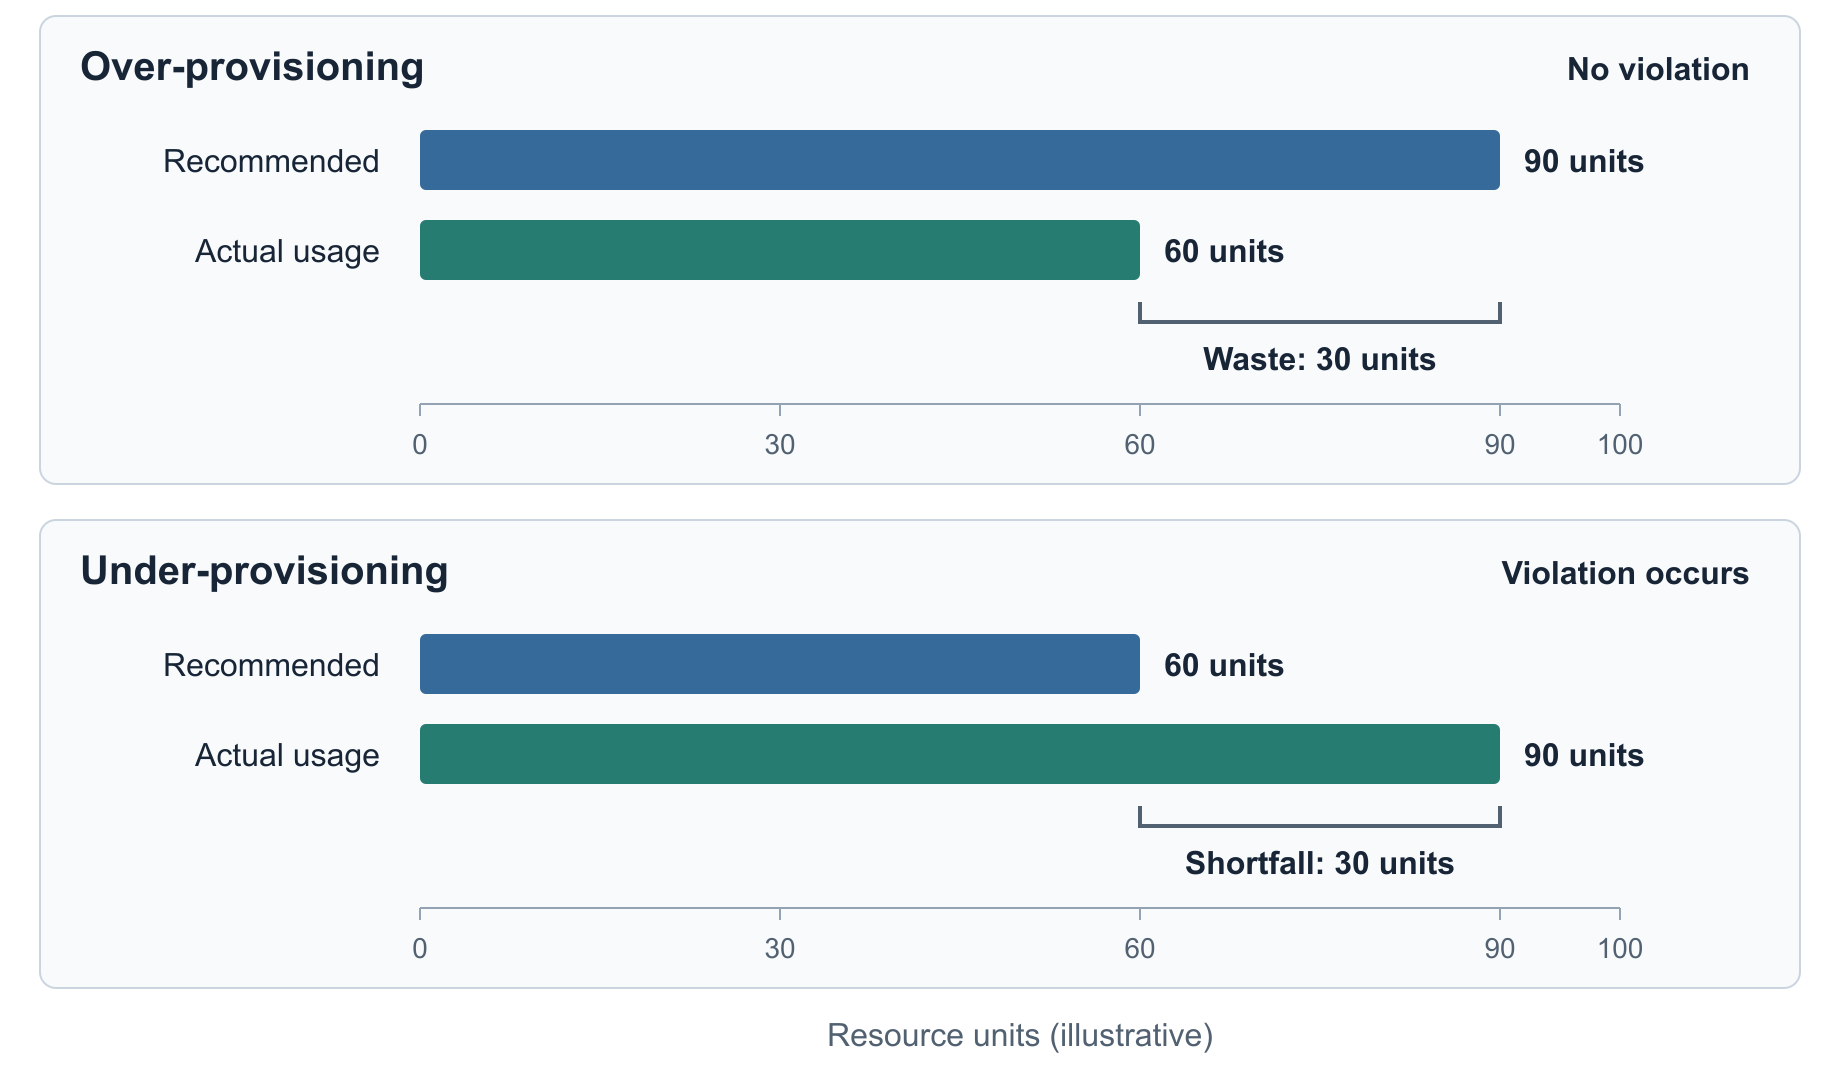
\includegraphics[width=0.92\linewidth]{figures/fig_4_2.png}
\caption{Waste and shortfall for an over-provisioned and an under-provisioned run (illustrative values)}\label{fig:4.2}
\end{figure*}

A row with a missing actual value or recommendation is unknown for that resource, is excluded from that resource's denominator and is never counted as a success; counting unknown rows as successes would make every policy look safer and would favour policies that produce missing recommendations. CPU and memory have separate denominators, and every rate is reported with its denominator. The capability profile decides what may be reported and how it is labelled. Alibaba CPU results are labelled as average-usage sizing, and the combined violation rate is reported only for Google, because on Alibaba it would combine an average-based CPU result with a peak-based memory result and have no clear meaning.

The evaluator computes metrics but never ranks or selects, so the same scoring code is applied to validation and test and to every policy, whatever rule chose it. All policies are compared on the same rows, a population frozen before any scoring, so that differences reflect the policies rather than the rows each could score. On Google, the population contains rows with both targets; on Alibaba, rows with at least one target, each resource evaluated over its own valid rows, because requiring both targets would discard valid memory evaluations whenever CPU is missing. Sensitivity analyses test whether conclusions depend on particular subsets without changing any decision: on Alibaba, rows whose next run was submitted in the same second, roles with more than one instance, and a weighting that counts each recurring workload equally, which tests whether a few very large workloads dominate; on Google, validation restricted to targets within the validation period, which measures the effect of the missing split isolation.

Repeatedly evaluating design choices against the same data and adjusting them overfits that data even when no single step looks improper, so the test set is used exactly once, after every decision has been frozen (Fig.~\ref{fig:4.3}). The training set is used to fit the ML models; the baselines are not fitted, because each row's baseline values come from its own point-in-time history. The validation set is used only to choose among policies, history thresholds and models. All selection decisions are then written to a decision manifest together with the checksums of every input, the code commit and the library versions; on Alibaba the baseline selection record is written before the test table is opened. The final test reads the test targets for the first time, scores all seven policies once and writes a run record; a second run is refused. A rerun is permitted only to correct a documented defect, whose reason is recorded, with every locked decision unchanged and the original results preserved. The procedure plays the role of pre-registration in experimental science: the analysis is fixed before the outcome is seen.

\begin{figure*}[!t]
\centering
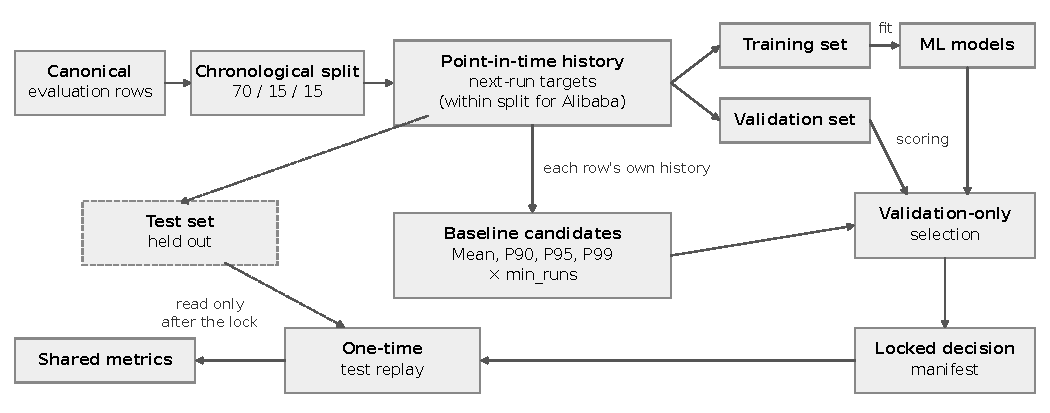
\includegraphics[width=0.92\linewidth]{figures/fig_4_3.pdf}
\caption{Time-ordered selection and final test}\label{fig:4.3}
\end{figure*}

\subsection{Artifact and Presentation Layer Design}\label{sec:4.4}

Each stage reads files written by earlier stages and writes its own (Fig.~\ref{fig:4.4}). Keeping every intermediate result as a file makes each stage inspectable and independently rerunnable, and allows any result to be shared and checked without rerunning the pipeline.

\begin{figure*}[!t]
\centering
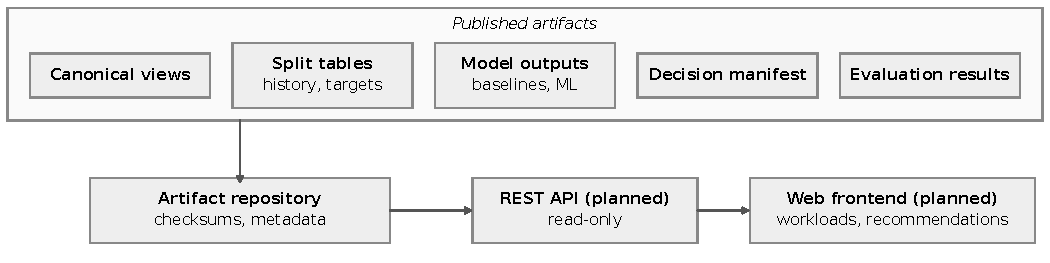
\includegraphics[width=0.92\linewidth]{figures/fig_4_4.pdf}
\caption{Artifact repository and presentation layer}\label{fig:4.4}
\end{figure*}

On Alibaba GPU 2020, every published output folder contains a checksum file listing the SHA-256 hash of each file, and each stage recomputes its inputs' hashes before running and stops if any differs, so a result can only be produced from the exact inputs it records. Outputs are written to a staging folder and moved into place only after all checks pass, so an interrupted run never leaves a partial output, and the raw source tables are verified against checksums committed with the code, so anyone who downloads the public trace can confirm they hold identical data. The Google pipeline, run as notebooks, applies these checks where they matter most for the results: its decision manifest records the hash of every input to the final test, including the split tables, ML predictions, locked models and evaluation code, and the final test refuses to run if any has changed. Each output also records the code commit and library versions, and all final runs use one locked software environment, because model results can change with library versions. Together with the decision manifest, these records make every reported number traceable to the data, code, environment and decisions behind it.

Tables are stored in Parquet, which preserves column types, including nullable integers and strings, so missing values survive every stage unchanged; CSV would not distinguish a missing value from an empty string. Metadata, selection records and manifests are stored in JSON and reported result tables in CSV. Raw and intermediate data remain local because of their size, while code, documentation, configuration and final results are versioned in the project repository.

The presentation layer is designed but not yet implemented (Section~\ref{sec:8.3}). A REST API exposes the published recommendations and evaluation results over HTTP in JSON, organized by dataset, workload and policy, and a web frontend built on it lets developers look up a workload, see its recommended CPU and memory under each policy and compare policies. The API is read-only: it serves only published, locked results and never runs the pipeline or modifies an artifact, so developers see exactly what was evaluated. Because it depends only on published files, it is decoupled from the pipeline and can be developed and deployed independently. Units and dataset labels, such as the fact that Alibaba CPU results describe average usage, are returned with each result, so the frontend never presents a value without the information needed to interpret it. Deployment is described in Section~\ref{sec:8}.

\subsection{Summary of Dataset-Specific Design Choices}\label{sec:4.5}

The design is shared across datasets wherever possible, but some choices must follow differences in what the traces record. Table~\ref{tab:4.1} summarizes these choices, which matter for interpreting the results in Section~\ref{sec:7}.

\begin{table*}[!t]
\centering
\footnotesize
\caption{Design choices that differ between the datasets}\label{tab:4.1}
\begin{tabular}{>{\raggedright\arraybackslash}p{0.276\linewidth}>{\raggedright\arraybackslash}p{0.225\linewidth}>{\raggedright\arraybackslash}p{0.409\linewidth}}
\hline
\textbf{Design choice} & \textbf{Google ClusterData 2019} & \textbf{Alibaba GPU 2020} \\ \hline
Evaluation unit & Full workload occurrence & One task role within one job, per instance \\
CPU target & Next occurrence's peak & Next role occurrence's lifetime average \\
Memory target & Next occurrence's peak & Next role occurrence's per-instance peak \\
Primary resource & CPU and memory & Memory \\
Targets kept within one split & No (known limitation) & Yes \\
Baseline ranking & Combined violation first & Memory violation first \\
Hybrid safeguard & P95, fixed in advance & Baseline selected on validation \\
Evaluation population & Rows with both targets & Rows with at least one target \\
\hline
\end{tabular}
\end{table*}
